% SPACE 2026 submission.
%
% Format, from the call for papers: official LNCS template with unmodified
% margins, at most 20 pages at 10 point INCLUDING bibliography and appendices,
% and double-blind review, so the submission must be anonymised.
\documentclass[runningheads]{llncs}

% *** MATH PACKAGES ***
\usepackage{amsmath}
% *** PDF, URL AND HYPERLINK PACKAGES ***
\usepackage{url}
\usepackage{algorithm}
\usepackage{algpseudocode}
% Concurrent-branch blocks: the deployed authentication evaluates the three
% factors in parallel, so the pseudocode needs a parallel construct rather than
% nested conditionals.
\algblockdefx[PARALLEL]{Parallel}{EndParallel}{\textbf{in parallel do}}{\textbf{end parallel}}
\algblockdefx[BRANCH]{Branch}{EndBranch}[1]{\textbf{branch} #1\textbf{:}}{\textbf{end branch}}
\usepackage{titlesec}
\usepackage{array}
\usepackage{graphicx}
\usepackage{multirow}
\usepackage{enumitem}
\usepackage{rotating}
\usepackage{amssymb}

\usepackage[center]{caption}

\usepackage{booktabs}
\usepackage{multirow}
\usepackage{pifont}
\newcommand{\xmark}{\ding{55}}
\newcommand{\ymark}{\ding{113}}
% Table 2 previously wrote \xmark both for "this system does not do it" and for
% "the paper does not say". Those are different claims about someone else's
% work, and only one of them is ours to make.
\newcommand{\nrmark}{\textit{n.r.}}
\graphicspath{ {./} {./Figures/} }

\usepackage{graphicx}  %needed to include png, eps figures
\usepackage{float}  % used to fix location of images i.e.\begin{figure}[H]
\usepackage{placeins}
\usepackage{tikz}
\usetikzlibrary{arrows.meta,positioning}

\usepackage{xcolor}

% Clickable links for the recent-literature comparison (loaded last).
\usepackage[hidelinks]{hyperref}

% ---------------------------------------------------------------------------
% Generated result macros.
%
% results.tex comes from the recognition-accuracy harness and attacks.tex from
% the presentation-attack harness. Both are written by those tools and are never
% edited by hand, so no number in this paper is retyped from a console. Copy them
% next to this file after a run.
%
% The \providecommand fallbacks below fire only for macros the generated files
% did not define, so the document still compiles before a harness has been run
% and every unmeasured quantity prints as "n/a" rather than as a plausible
% invented value.
% ---------------------------------------------------------------------------
% The flags let prose that must read as a finished sentence -- the abstract and
% the conclusion -- switch between the measured claim and an explicit statement
% that the measurement is outstanding, instead of printing "n/a" mid-sentence.
\newif\ifresultsready
\newif\ifattacksready
\InputIfFileExists{results.tex}{\resultsreadytrue}{\resultsreadyfalse
  \typeout{results.tex absent: accuracy values print as n/a}}
\InputIfFileExists{attacks.tex}{\attacksreadytrue}{\attacksreadyfalse
  \typeout{attacks.tex absent: attack values print as n/a}}

\providecommand{\EvalCorpusName}{n/a}
\providecommand{\EvalSubjects}{n/a}
\providecommand{\EvalSessions}{n/a}
\providecommand{\EvalGenuinePairs}{n/a}
\providecommand{\EvalImpostorPairs}{n/a}
\providecommand{\EvalFaceEER}{n/a}
\providecommand{\EvalFaceAUC}{n/a}
\providecommand{\EvalFaceEERTau}{n/a}
\providecommand{\EvalFaceFAR}{n/a}
\providecommand{\EvalFaceFRR}{n/a}
\providecommand{\EvalVoiceEER}{n/a}
\providecommand{\EvalVoiceAUC}{n/a}
\providecommand{\EvalVoiceEERTau}{n/a}
\providecommand{\EvalVoiceFAR}{n/a}
\providecommand{\EvalVoiceFRR}{n/a}
\providecommand{\EvalFusedFAR}{n/a}
\providecommand{\EvalFusedFRR}{n/a}
\providecommand{\EvalPredFusedFAR}{n/a}
\providecommand{\EvalPredFusedFRR}{n/a}
\providecommand{\EvalChallengeFRR}{n/a}
\providecommand{\EvalChallengeTrials}{n/a}
\providecommand{\EvalAccuracyRows}{\multicolumn{8}{c}{\textit{harness not yet run}}\\}
\providecommand{\EvalIndependenceRows}{\multicolumn{4}{c}{\textit{harness not yet run}}\\}
\providecommand{\EvalCrossDeviceRows}{\multicolumn{5}{c}{\textit{harness not yet run}}\\}
\providecommand{\AttackChallengeSpace}{100{,}000}
\providecommand{\AttackSubjects}{n/a}
\providecommand{\AttackControlValid}{n/a}
\providecommand{\AttackRows}{\multicolumn{6}{c}{\textit{harness not yet run}}\\}
% Per-attack macros used by the attack/defence mapping table. The names match
% what attack_suite.mjs derives from each attack id.
\providecommand{\AttackReplayASR}{n/a}
\providecommand{\AttackReplayN}{n/a}
\providecommand{\AttackSpliceVictimFaceASR}{n/a}
\providecommand{\AttackSpliceVictimFaceN}{n/a}
\providecommand{\AttackSpliceVictimVoiceASR}{n/a}
\providecommand{\AttackSpliceVictimVoiceN}{n/a}
\providecommand{\AttackPhotoLiveVoiceASR}{n/a}
\providecommand{\AttackPhotoLiveVoiceFaceASR}{n/a}
\providecommand{\AttackPhotoLiveVoiceN}{n/a}
\providecommand{\AttackPhotoArchivedAudioASR}{n/a}
\providecommand{\AttackPhotoArchivedAudioN}{n/a}
\providecommand{\AttackVoiceCloneASR}{n/a}
\providecommand{\AttackVoiceCloneVoiceASR}{n/a}
\providecommand{\AttackVoiceCloneN}{n/a}
\providecommand{\AttackFaceSwapASR}{n/a}
\providecommand{\AttackFaceSwapFaceASR}{n/a}
\providecommand{\AttackFaceSwapN}{n/a}
\providecommand{\AttackControlGenuineASR}{n/a}
\providecommand{\AttackControlGenuineN}{n/a}

\begin{document}

\title{Secure User Authentication Scheme Using Multimodal Biometrics}

% Double-blind submission: author names and the institution are withheld, and
% the authors' own earlier work is cited in the third person throughout.
\author{Anonymous Author(s)}
\institute{Submitted for double-blind review}

\maketitle

\begin{abstract}
Authentication systems increasingly require stronger protection against credential theft, replay, and biometric spoofing while remaining practical to deploy. Although multimodal biometrics can improve authentication robustness, conventional approaches often require separate acquisition of multiple traits, increasing hardware requirements, cost, and user interaction. This paper presents a deployable multimodal authentication system that derives face, voice, and a dynamic challenge response factor from a single real time video recording. During login, the user records a video while responding to a server issued CAPTCHA. Face verification and speaker verification are performed using learned biometric embeddings and cosine similarity based decisions, while the spoken response is transcribed and validated against the session specific challenge. The three factors are evaluated concurrently and combined using a conjunctive decision rule, granting access only when all verification factors succeed.

The system therefore enables single sensor acquisition of multiple authentication factors without requiring dedicated biometric hardware for each modality. For privacy, uploaded recordings are reduced to templates and are not retained as persistent media, the resulting templates are encrypted under per user keys, and the corresponding key material is held in a separate vault, so recovering a template requires compromising both stores. Speech to text is performed on premises, so the login audio does not leave the deployment.
%
% Measured claims. The macros are written by the evaluation and attack
% harnesses; the \else branches state plainly that a measurement is outstanding
% rather than leaving a number-shaped gap in the sentence.
\ifresultsready
We evaluate recognition accuracy on \EvalCorpusName, forming genuine pairs only across different sessions of the same subject (\EvalGenuinePairs{} pairs) and impostor pairs across different subjects (\EvalImpostorPairs{} pairs), and report an Equal Error Rate (EER) of \EvalFaceEER\% for the face factor and \EvalVoiceEER\% for the speaker factor, together with False Acceptance Rate (FAR) and False Rejection Rate (FRR) at the deployed operating points and the measured cost of the challenge factor's own false rejections (\EvalChallengeFRR\%).
\else
Recognition accuracy is evaluated on a public audio visual corpus using an automated harness that applies the deployed matcher paths, forms genuine pairs only across different sessions of the same subject and impostor pairs across different subjects, and reports FAR, FRR, EER, ROC, DET and AUC; the corpus run is outstanding and no accuracy figure is claimed here.
\fi
\ifattacksready
Against presentation attacks the system is evaluated directly: replay of archived recordings, face--voice splicing in both directions, photograph and screen replay, synthetic speech, and face swapping are each mounted against the deployed decision rule and reported as attack success rates, per factor and for the system as a whole.
\else
A presentation attack harness mounts replay, face--voice splicing in both directions, photograph and screen replay, synthetic speech and face swapping against the deployed decision rule, reporting each as an attack success rate per factor and for the system; those runs are outstanding.
\fi
The evaluation also identifies template extraction and model loading as the main contributors to authentication latency. The architecture is presented together with an explicit adversary model and a statement of the attacks it does not defend against, notably real time relay and real time responsive deepfakes.

\keywords{Multimodal biometrics \and Authentication \and Challenge response \and Face verification \and Speaker verification \and Replay resistance \and Template protection}
\end{abstract}

\noindent\textbf{Nomenclature:} FAR, False Acceptance Rate; FRR, False Rejection Rate; EER, Equal Error Rate; ROC, Receiver Operating Characteristic; DET, Detection Error Tradeoff; AUC, Area Under the Curve; ASR, Attack Success Rate; PAD, Presentation Attack Detection; STT, Speech to Text; TTL, Time to Live; MITM, Man in the Middle.

\section {Introduction}

% The knowledge/possession/inherence taxonomy and its figure were cut for the
% LNCS page limit: this venue's readers do not need authentication factors
% introduced, and the space is better spent on the evaluation.
Authentication factors are conventionally drawn from what the user knows, what
they possess, and what they are. Knowledge factors dominate deployed systems and
are also their weakest link, since a password can be exposed, guessed, stolen, or
reused. Biometric factors bind authentication to a characteristic of the person
instead, and combining several traits reduces reliance on any one of them --- at
the cost, in most multimodal deployments, of a separate sensor per trait.

This work concerns user to device authentication and uses face and voice as its
biometric factors, both derived from a \emph{single} commodity recording, and
combines them with a dynamic challenge response factor derived from the same
recording. Access is granted only when all three verification decisions succeed.

\subsection{Research problem and motivation}
Researchers are trying to find a more secure and robust authentication mechanism to combat security threats and prevent the system from cyber attacks. Single factor authentication can be vulnerable to compromise of its single authentication factor, motivating the use of multiple complementary factors. Passwords may be exposed, guessed, stolen, or reused through attacks such as guessing and brute force attacks. MFA  and passwordless authentication is gaining popularity and becoming the current trend. In the previous subsection, the benefits of biometric authentication are discussed and how multimodal biometric authentication can be a viable solution. Multimodal biometrics, which involves more than one biometric trait, is a secure and effective authentication mode. All the schemes based on multimodal biometrics involve some problems like
\begin{itemize}
\item interacting with different devices to provide biometric identity
\item The extra cost involved in purchasing devices
\end{itemize}
So, \textcolor{black}{many multimodal biometric systems use separate acquisition modalities or dedicated sensing hardware, which can increase deployment complexity and cost. The proposed scheme instead combines parallel acquisition of biometrics from a commodity camera and microphone with binding of that acquisition to a fresh server issued challenge}.

{\color{black}
\subsection{Major Contributions}\label{sec:contrib}
The individual components used here --- deep face embeddings, speaker embeddings, spoken challenges, authenticated encryption --- are established, and no novelty is claimed for any of them in isolation. What this paper contributes is a single capture, challenge bound face and voice authenticator that is built, deployed, and then \emph{measured} on the two axes such a system is normally asserted to satisfy rather than shown to: recognition accuracy, and resistance to presentation attack. Each contribution below names the result that supports it.

\begin{enumerate}[leftmargin=*,itemsep=2pt,topsep=3pt]
\item \textbf{A single sensor, three factor authenticator with a conjunctive decision rule.} Face, speaker, and a session specific spoken challenge are all derived from one commodity camera and microphone recording, evaluated concurrently, and combined by the AND rule of~(\ref{eq:fusion}), so compromise of any single factor cannot grant access. \emph{Result:} Section~\ref{sec:accuracy} reports an EER of \EvalFaceEER\% for the face factor and \EvalVoiceEER\% for the speaker factor over \EvalGenuinePairs{} genuine and \EvalImpostorPairs{} impostor pairs, with FAR and FRR at the deployed thresholds and at the EER threshold.

\item \textbf{A measured account of what the challenge actually buys.} The challenge is server generated, withheld from the client, single use, and short lived, which is what defeats archived media. \emph{Result:} Section~\ref{sec:attacks} reports the measured success rate of replaying an archived login recording against a fresh challenge, and Section~\ref{sec:threat} bounds the residual coincidence probability at $1/\AttackChallengeSpace$ per attempt from the challenge space.

\item \textbf{An attack evaluation that reports per factor as well as system outcomes.} Replay, face--voice splicing in both directions, photograph and screen replay, synthetic speech, and face swapping are mounted against the deployed decision rule. \emph{Result:} Section~\ref{sec:attacks} shows which factor stops each attack --- including attacks that fully defeat one factor while the system still denies access, which is the evidence that the conjunctive rule is doing work rather than being assumed to.

\item \textbf{An honest cost accounting for the third factor.} Conjunctive fusion moves error onto the user, and the spoken challenge is the weakest link in practice. \emph{Result:} Section~\ref{sec:accuracy} reports the challenge factor's own false rejection rate (\EvalChallengeFRR\% over \EvalChallengeTrials{} controlled trials) and Section~\ref{sec:outcomes} shows it dominating observed login failures in deployment; Section~\ref{sec:accuracy} also compares the measured fused error against the independence approximation of~(\ref{eq:farsys}) and~(\ref{eq:frrsys}).

\item \textbf{A storage design whose compromise requirements are stated precisely.} Raw recordings are destroyed after template extraction; templates are encrypted under per user keys whose wrapped forms live in a separate vault under a pseudonymous index. \emph{Result:} Section~\ref{sec:threat} states what each of adversaries A1--A4 obtains, and is explicit that encrypted embeddings are not cancelable templates and do not prevent template inversion by an adversary who obtains the plaintext.

\item \textbf{Purpose bound enrollment and an on premises speech pipeline.} A normal enrollment grant cannot overwrite an existing template; replacement requires a \texttt{reenroll} grant issued only after successful three factor verification. Transcription runs on the deployment's own hardware, so the login audio --- which carries both the challenge response and the user's voice --- is never sent to a third party.
\end{enumerate}

The rest of this paper is organised as follows. Section~\ref{sec:related} reviews the related literature and Section~\ref{sec:proposed} presents the system, its decision rule, and its threat model. Section~\ref{sec:eval} reports recognition accuracy, the attack evaluation, and deployment measurements. Section~\ref{sec:future} outlines future work and Section~\ref{sec:conclusion} concludes.
}

\section{Related Work}\label{sec:related}
Biometric authentication has evolved from single trait verification towards multi factor and multimodal approaches that combine biometric information with additional security mechanisms. Marasco and Albanese \cite{IEEEtran37} proposed FingerPIN, a multi factor authentication approach that combines knowledge and inherence factors through a fingerprint based personal identification number (PIN), while an improved version of the scheme was subsequently introduced to strengthen security and usability \cite{IEEEtran38}. Li and Hwang \cite{IEEEtran32} proposed a remote biometric authentication scheme based on biometric verification, one way hashing, and smart card technology. Das \cite{IEEEtran33} later proposed an improved scheme, however, it was shown to lack resistance against offline password guessing and privileged insider attacks and did not provide user anonymity. To address these limitations, Lee and Hsu \cite{IEEEtran56} introduced an alternative approach based on extended chaotic maps.

Other studies have investigated the integration of biometric traits with cryptographic mechanisms and machine learning techniques. Jagadiswary and Saraswady \cite{IEEEtran58} proposed an authentication scheme combining RSA asymmetric cryptography with biometric traits such as fingerprints, retina scans, and finger-vein patterns. Finger vein based authentication and identification have also received attention, including approaches focused on improving vein image quality and reducing noise during feature extraction \cite{IEEEtran61}, as well as convolutional neural network based biometric identification systems \cite{IEEEtran62}. These studies demonstrate the applicability of cryptographic and learning based techniques for strengthening biometric authentication, however, they primarily focus on different biometric modalities and acquisition settings from those considered in the present work.

More recent research has increasingly explored multimodal authentication through different combinations of biometric traits and fusion strategies. Hammad et al.\ \cite{r1} proposed sequential and parallel multimodal authentication systems using ECG and fingerprint biometrics and employed CNN and Q-Gaussian multi support vector machine (QG-MSVM) based processing. Kim and Hong \cite{r4} combined teeth images and voice biometrics, where individual matching scores were integrated using weighted score level fusion. Ahamed et al.\ \cite{r2} proposed an AI based device level authentication model using ECG and PPG signals, while \cite{r3} investigated the combination of fingerprint, face, and iris biometrics using different machine learning based fusion and classification approaches. Collectively, these studies demonstrate the benefits of combining multiple biometric traits, however, they differ in terms of the biometric modalities considered, acquisition requirements, fusion strategies, and security mechanisms.

The proposed work differs from these approaches by integrating facial verification, speaker verification, and a session specific spoken challenge within a unified passwordless authentication framework. Rather than relying solely on biometric score fusion, the system independently verifies the facial biometric, speaker biometric, and challenge response and applies a strict decision level AND rule for the final authentication decision. The dynamic challenge additionally mitigates the reuse of previously recorded authentication media by requiring a response to a fresh challenge associated with the current authentication attempt. The proposed architecture also incorporates concurrent factor evaluation, privacy oriented template only storage with authenticated encryption, and an authorized enrollment mechanism. A more detailed comparison with recent end to end biometric authentication systems follows the proposed system discussion and is summarized in Table~\ref{tab:recentsec}.

\long\def\recentcomparison{%
{\color{black}

\subsection{\textcolor{black}{Comparison with Recent Authentication Systems (2024--2026)}}\label{sec:recent}
This work presents an end to end multimodal biometric authentication system and therefore, the comparison is restricted to recent studies that explicitly implement a biometric authentication or verification procedure. Table~\ref{tab:recentsec} compares the proposed scheme with five relevant authentication systems published between 2024 and 2026 \cite{jha2024featurefusion,aanjankumar2025smartcity,jha2025ensemble,chen2026twostep,jha2025challenge}. Works primarily focused on biometric recognition, presentation attack detection, cross-modal attacks, or template protection techniques \cite{alharbi2023facevoice,mandalapu2021avpad,jiang2024foice,rathgeb2023btp,zhao2023deephash} are considered supporting literature rather than directly comparable authentication systems. In Table~\ref{tab:recentsec}, \checkmark\ denotes a property the cited work states it supports and \xmark\ a property it states it does not, while \nrmark\ denotes a property the cited work simply does not report. The distinction matters: most of these systems were not written to answer questions about template storage or challenge lifecycle, and marking silence as absence would assert something about their work that we are not entitled to assert. For the proposed system, ``challenge only'' denotes challenge response evidence rather than a dedicated Presentation Attack Detection or deepfake detector. Table~\ref{tab:recentacc} separately records the accuracy each work reports, on its own dataset, wherever it reports one.

\vspace{0.5\baselineskip}
\begin{table}[!t]
\caption{\textcolor{black}{Comparison of Security and Authentication Properties with Recent Systems (2024--2026)}}
\label{tab:recentsec}
\centering
\renewcommand{\arraystretch}{1.5}
\footnotesize
\setlength{\tabcolsep}{2.5pt}
\begin{tabular}{|>{\raggedright\arraybackslash}p{2.7cm}|*{8}{>{\centering\arraybackslash}p{1.38cm}|}>{\centering\arraybackslash}p{1.65cm}|}
\hline
\textbf{Work} & \textbf{Liveness / PAD} & \textbf{Replay Prot.} & \textbf{Dyn.\ Chall.} & \textbf{Phish / MITM} & \textbf{Templ.\ Prot.} & \textbf{Encr.} & \textbf{Unlink./ Pseud.} & \textbf{Server dec.} & \textbf{Raw media permanently retained} \\ \hline
Jha et al.~\cite{jha2024featurefusion} & \checkmark & \xmark & \xmark & \nrmark & \nrmark & \nrmark & \nrmark & \nrmark & \nrmark \\ \hline
Aanjankumar et al.~\cite{aanjankumar2025smartcity} & \checkmark & \checkmark & \xmark & \checkmark & \checkmark & \checkmark & \nrmark & \nrmark & \nrmark \\ \hline
Jha et al.~\cite{jha2025ensemble} & \checkmark & \xmark & \xmark & \nrmark & \nrmark & \nrmark & \nrmark & \nrmark & \nrmark \\ \hline
Chen et al.~\cite{chen2026twostep} & \xmark & \xmark & \xmark & \nrmark & \nrmark & \nrmark & \nrmark & \nrmark & \nrmark \\ \hline
Jha et al.~\cite{jha2025challenge} & \checkmark & \checkmark & \checkmark & \nrmark & \nrmark & \nrmark & \nrmark & \checkmark & \nrmark \\ \hline
\textbf{Proposed Scheme} & challenge only & \checkmark & \checkmark & \xmark & \checkmark & \checkmark & \checkmark & \checkmark & No, template only \\ \hline
\end{tabular}

\vspace{0.3\baselineskip}
{\footnotesize \checkmark\ stated as supported \quad \xmark\ stated as not supported \quad \nrmark\ not reported by the cited work.
The first three columns describe the authentication method itself and are read from each work's design. The remaining columns describe storage and deployment properties that most recognition-oriented papers do not discuss; silence there is recorded as \nrmark\ rather than as absence.}
\end{table}

% ---------------------------------------------------------------------------
% TO COMPLETE BEFORE SUBMISSION: fill the cells below from each cited paper's
% own reported evaluation. Leave \nrmark wherever the paper genuinely reports
% no such figure -- do not infer, convert, or estimate a number on another
% group's behalf. The datasets differ, so these are context for the proposed
% system's numbers, never a like-for-like ranking.
% ---------------------------------------------------------------------------
\begin{table}[!t]
\caption{Accuracy as reported by each cited work, on its own dataset. The evaluation corpora, modalities, and protocols differ across rows, so these figures are context rather than a common benchmark; \nrmark\ marks a figure the cited work does not report.}
\label{tab:recentacc}
\centering
\renewcommand{\arraystretch}{1.18}
\setlength{\tabcolsep}{4pt}
\footnotesize
\begin{tabular}{llrrl}
\toprule
\textbf{Work} & \textbf{Modalities} & \textbf{Subjects} & \textbf{Reported EER / accuracy} & \textbf{Dataset} \\
\midrule
Jha et al.~\cite{jha2024featurefusion} & Face + speech & \nrmark & \nrmark & \nrmark \\
Aanjankumar et al.~\cite{aanjankumar2025smartcity} & Face & \nrmark & \nrmark & \nrmark \\
Jha et al.~\cite{jha2025ensemble} & Multimodal & \nrmark & \nrmark & \nrmark \\
Chen et al.~\cite{chen2026twostep} & Face + voice & \nrmark & \nrmark & \nrmark \\
Jha et al.~\cite{jha2025challenge} & Face + voice + challenge & \nrmark & \nrmark & \nrmark \\
\midrule
\textbf{Proposed scheme} & Face + voice + challenge & \EvalSubjects & EER \EvalFaceEER\% face, \EvalVoiceEER\% voice & \EvalCorpusName \\
\bottomrule
\end{tabular}
\end{table}

Existing studies demonstrate the use of multimodal biometrics, liveness detection, challenge response mechanisms, and biometric template protection. The proposed work does not claim novelty for these individual components in isolation. Instead, its contribution lies in integrating facial verification, speaker verification, and a session specific spoken challenge within a single authentication architecture. The system further combines concurrent factor evaluation with strict decision level AND fusion, template only storage protected using authenticated encryption, pseudonymous template naming, enrollment binding, and explicit challenge lifecycle controls. As summarized in Table~\ref{tab:recentsec}, the closest challenge response multimodal system \cite{jha2025challenge} employs a spoken challenge for liveness, whereas the proposed architecture additionally incorporates server side single use challenge management, independent per factor decisions combined through conjunctive fusion, protected template storage, and enrollment authorization.

The privacy and security advantage claimed in this comparison is the combination of protected templates, authenticated encryption, and unlinkability through pseudonymous naming. It is not a storage size comparison, because the compared works do not report comparable per user storage measurements. Raw enrollment and authentication recordings are not retained as permanent biometric records by the proposed system; for the compared systems, raw media retention is marked as not stated where the cited work does not specify it.

What distinguishes this work from the row above it is not the component list but what is demonstrated about the assembled system. The closest challenge response multimodal system~\cite{jha2025challenge} uses a spoken challenge as liveness evidence and reports recognition accuracy; it does not report what happens when an adversary actually replays, splices, or synthesises the media it is shown. Section~\ref{sec:attacks} reports exactly that, per factor and for the system, against the deployed decision rule, and Section~\ref{sec:accuracy} pairs it with corpus level EER, AUC, ROC and DET for each factor and with the challenge factor's own cost to legitimate users. Consistent with the threat model, the challenge response mechanism defeats reuse of previously recorded media but claims nothing against real time relay or a real time deepfake able to answer an unpredictable challenge inside the validity window.

}
}

\section{Proposed System and Methodology}\label{sec:proposed}
The proposed scheme is a multimodal biometric authentication system that combines face verification, speaker verification, and a dynamic challenge-response factor. All three factors are derived from a single real time video recording, allowing facial and voice information to be acquired simultaneously while the user speaks a server issued challenge. Authentication succeeds only when the face, voice, and challenge response decisions are all positive under a conjunctive decision rule.

During registration, the user's biometric representations are extracted from the submitted recording and retained as encrypted templates rather than as raw biometric media. Each template is protected using an independent per user encryption key, while the corresponding protected key material is maintained separately in the key vault database. During login, a newly submitted recording is used to derive face and voice representations and to validate the spoken challenge. The biometric representations are compared with the enrolled references, while the transcribed response is verified against the challenge issued for the authentication attempt.

The dynamic challenge provides freshness to the authentication attempt and helps prevent simple reuse of previously recorded authentication responses. The three verification results are combined using AND logic, therefore, access is granted only when all three factors are successfully verified.

The proposed authentication scheme consists of three phases:
\begin{itemize}
\item Registration Phase
\item Login and Challenge Issuance Phase
\item Authentication Phase
\end{itemize}

\long\def\technicalsubsections{%
{\color{black}

\subsection{\textcolor{black}{System Model and Decision Rule}}\label{sec:model}
Let $V_r$ and $V_l$ denote the videos acquired during registration and login respectively, and let $C$ denote the CAPTCHA string issued by the server for the current session. Three decisions are derived from the single login stream:
\begin{itemize}
\item a face decision obtained by scoring the login recording's per frame face embeddings against the enrolled face embedding at a threshold $\tau_f$;
\item a voice decision obtained by scoring the login speaker embedding against the enrolled speaker embedding at a threshold $\tau_a$;
\item a challenge decision obtained by transcribing the login audio and comparing the transcript with $C$.
\end{itemize}
Both biometric factors are scored by \emph{similarity} rather than distance. For an embedding $e\in\mathbb{R}^{d}$, the L2 (Euclidean) norm is
\begin{equation}
\lVert e\rVert_2=\left(\sum_{j=1}^{d}e_j^2\right)^{1/2}, \qquad \widehat e=\frac{e}{\lVert e\rVert_2}.
\label{eq:l2}
\end{equation}
L2 normalization therefore rescales an embedding to unit Euclidean norm. For two unit norm embeddings, $\langle \widehat e_1,\widehat e_2\rangle=\cos\theta$, so their inner product is exactly their cosine similarity. Let $e_r^{f}$ denote the normalized enrolled face embedding and $\{e_{l,i}^{f}\}_{i=1}^{n}$ the normalized per frame embeddings of the login recording, and let $e_r^{a}$ and $e_l^{a}$ denote the normalized enrolled and login speaker embeddings. Writing $T(\cdot)$ for the Speech to Text (STT) transform and $\mathcal{N}(\cdot)$ for the CAPTCHA normalization map, the factor decisions are
\begin{equation}
b_f = \mathbb{I}\Big[\operatorname{median}_{i}\big\langle e_r^{f},\, e_{l,i}^{f}\big\rangle \;\geq\; \tau_f\Big],
\label{eq:face}
\end{equation}
\begin{equation}
b_a = \mathbb{I}\Big[\big\langle e_r^{a},\, e_l^{a}\big\rangle \;\geq\; \tau_a\Big],
\label{eq:voice}
\end{equation}
\begin{equation}
b_c = \mathbb{I}\Big[\exists\, t \in T(A_l): \mathcal{N}(t) = \mathcal{N}(C)\Big],
\label{eq:captcha}
\end{equation}
where $\mathbb{I}[\cdot]$ is the indicator function. The face score is the \emph{median} of the per frame similarities rather than the mean, so that a minority of degraded frames (motion blur, partial pose, transient occlusion) cannot move the verdict. The challenge decision accepts if \emph{any} transcription hypothesis matches after normalization, because the speech to text stage returns a ranked list of alternatives and the correct reading of a spoken digit string is frequently not the top ranked one.
Fusion is performed at the decision level under a conjunctive rule,
\begin{equation}
D = b_f \wedge b_a \wedge b_c ,
\label{eq:fusion}
\end{equation}
A conjunctive rule is used so that compromise or successful spoofing of a single factor cannot independently produce a positive authentication decision. All three factors are evaluated concurrently and fused only after their verdicts are available. The rejection response is identical regardless of the failing factor, and per-factor outcomes are retained only in server side logs, reducing disclosure of factor specific information to the client.

If the three factors failed independently, the conjunctive system would satisfy
\begin{equation}
\label{eq:farsys}
\mathrm{FAR}_{\mathrm{sys}}\approx \mathrm{FAR}_{f}\mathrm{FAR}_{a}\mathrm{FAR}_{c},
\end{equation}
\begin{equation}
\label{eq:frrsys}
\mathrm{FRR}_{\mathrm{sys}}\approx 1-(1-\mathrm{FRR}_{f})(1-\mathrm{FRR}_{a})(1-\mathrm{FRR}_{c}).
\end{equation}
AND fusion therefore trades a lower False Acceptance Rate for a higher False Rejection Rate than any individual factor. Independence is an assumption rather than a property of this system: all three factors are derived from the \emph{same} recording, so a capture that is dark, brief, or noisy can degrade several of them at once, and their errors are then positively correlated. Section~\ref{sec:accuracy} therefore reports the measured fused error alongside the values~(\ref{eq:farsys}) and~(\ref{eq:frrsys}) predict, and treats the discrepancy as a result in its own right rather than as an approximation to be excused.

\begin{figure}[!t]
\centering
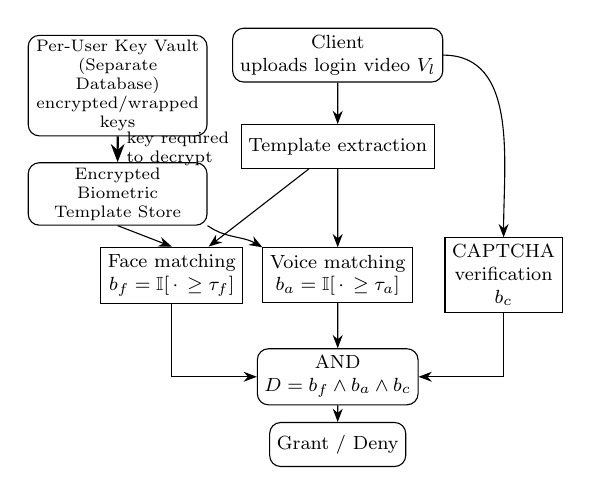
\begin{tikzpicture}[
scale=0.86,
transform shape,
font=\footnotesize,
>={Stealth[]},
box/.style={draw, rounded corners, align=center, inner sep=3pt, minimum height=6.5mm},
op/.style={draw, align=center, inner sep=3pt, minimum height=6.5mm},
storage/.style={draw, rounded corners, align=center, inner sep=2pt, font=\scriptsize, text width=25mm, minimum height=8mm}
]
\node[box] (client) at (0,0) {Client\\uploads login video $V_l$};
\node[op] (extract) at (0,-1.35) {Template extraction};
\node[storage] (vault) at (-3.25,-0.45) {Per-User Key Vault\\(Separate Database)\\encrypted/wrapped keys};
\node[storage] (store) at (-3.25,-2.05) {Encrypted Biometric\\Template Store};
\node[op] (face) at (-2.45,-3.25) {Face matching\\$b_f=\mathbb{I}[\,\cdot\,\ge\tau_f]$};
\node[op] (voice) at (0,-3.25) {Voice matching\\$b_a=\mathbb{I}[\,\cdot\,\ge\tau_a]$};
\node[op] (cap) at (2.45,-3.25) {CAPTCHA\\verification\\$b_c$};
\node[box] (and) at (0,-4.75) {AND\\$D=b_f\wedge b_a\wedge b_c$};
\node[box] (out) at (0,-5.75) {Grant / Deny};
% biometric branch
\draw[->] (client)--(extract);
\draw[->] (extract)--(face);
\draw[->] (extract)--(voice);
\draw[->, thick] (vault)--node[right, font=\scriptsize, align=left]{key required\\to decrypt} (store);
\draw[->] (store.south)--(face.north);
\draw[->] (store.south east) to[out=-35,in=150] (voice.north west);
% challenge branch runs concurrently, from the same recording
\draw[->] (client.east) to[out=0,in=90] (cap.north);
% fusion
\draw[->] (face) |- (and);
\draw[->] (voice) -- (and);
\draw[->] (cap) |- (and);
\draw[->] (and)--(out);
\end{tikzpicture}
\vspace{2mm}
\caption{\textcolor{black}{Deployed concurrent authentication architecture. The login video is processed through concurrent face, voice, and CAPTCHA verification branches. Enrolled biometric templates are retained only in encrypted form, while the corresponding wrapped per user keys are maintained in a separate key vault. The three verdicts are combined by the conjunctive rule in~(\ref{eq:fusion}), and access is granted only when all three pass.}}
\label{fig:concurrent}
\end{figure}

\subsection{\textcolor{black}{Feature Representations}}\label{sec:features}
\emph{Face.} The face verification factor uses a deep face recognition model to generate a 512 dimensional embedding for each detected face \cite{arcface}. Twelve frames are sampled by evenly spaced frame index from each recording, and facial embeddings are extracted from the valid detected faces. The detector aligns and crops each face to the recognition model input. The enrolled reference is the L2 normalized mean of the frame embeddings. During authentication, the per frame face representations are compared with the enrolled reference using cosine similarity and the median score is used in~(\ref{eq:face}). The face factor is accepted at $\tau_f=0.35$. This value is an inherited operating point. The observed genuine score of 0.8385 and impostor score of 0.0928 support separation on the available recordings, but do not constitute an EER calibration.

\emph{Voice.} The voice verification factor uses a 192 dimensional ECAPA TDNN speaker embedding \cite{ecapa}. Audio is resampled to 16 kHz mono before embedding extraction. The normalized speaker representation is compared with the enrolled reference using cosine similarity, as defined in~(\ref{eq:voice}). The voice factor is accepted at $\tau_a=0.30$, an operating point originally chosen from pilot observations in which the maximum cross speaker impostor cosine was approximately 0.256 and the genuine same speaker floor approximately 0.345; Section~\ref{sec:accuracy} revisits it against the corpus level distributions. An earlier MFCC distance statistic was discarded because it was not speaker discriminative at all: its impostor range (153.7 to 193.0) spanned its genuine range (172.8 to 178.8), so no threshold could separate the two populations.

\emph{Acquisition variability.} Device variation is partly absorbed by detector side face alignment, frame sampling by index rather than timestamp, median fusion of login face scores, cosine scoring of normalized embeddings, and audio conversion to 16 kHz mono. The browser requests ideal 1280 by 720 video at 30 frames per second and mono audio, with a one time fallback to unconstrained capture if negotiation fails. During enrollment only, a quality gate requires at least six usable sampled frames with a detected face of at least 80 by 80 pixels. The gate is not applied during login, where it could unnecessarily increase rejection of an already enrolled user. Per attempt width, height, frame rate, and platform metadata are retained in the benchmark log to support later cross device analysis. These mechanisms improve input consistency but do not establish cross device robustness, because no formal cross device experiment has yet been performed.

Section~\ref{sec:accuracy} sweeps each modality threshold over genuine pairs formed from different sessions of the same subject and impostor pairs formed from different subjects, and reports the threshold at each modality's Equal Error Rate alongside FAR and FRR at the deployed operating point.

\subsection{\textcolor{black}{Security Mechanisms}}\label{sec:security}
The proposed system incorporates multiple mechanisms to protect biometric data and the authentication workflow. During registration, the submitted video is processed to extract facial and voice biometric templates. The raw recording is not retained after successful processing, only the biometric representations required for subsequent verification are stored. This reduces the persistent exposure of reusable face and voice media and limits the amount of sensitive biometric data retained by the system.

Each enrolled user is assigned an independent cryptographically random 256 bit key that encrypts only that user's biometric template using AES-256-GCM. The per user key is not stored in plaintext with the biometric template or account data. Instead, it is stored in a separate key-vault database in encrypted form, where it is wrapped using a server side master key. The vault also uses a keyed pseudonymous index instead of storing usernames directly. Consequently, compromise of one user's template encryption key does not automatically expose the biometric templates of other users, and compromise of the template storage alone does not provide the corresponding decryption keys.

The system further protects the confidentiality and integrity of stored biometric data through authenticated encryption. During authentication, only the key associated with the requested user is retrieved and used to decrypt that user's template. The plaintext key exists only temporarily during the cryptographic operation and is cleared afterwards. Missing or tampered key material, as well as modified encrypted templates, cause the operation to fail rather than allowing authentication to continue.

The system also protects the association between an account and its biometric data during enrolment. Initial enrollment is authorized by a purpose bound \texttt{enroll} grant and is bound to the intended account through server controlled validation rather than client controlled information such as an uploaded filename. A normal enrollment grant cannot overwrite an existing enrolled template. Template replacement is available only through a purpose bound \texttt{reenroll} grant issued after successful three factor authentication, as described in Section~\ref{sec:lifecycle}.

During authentication, the server generates a dynamic challenge for each login attempt. The expected challenge value is not exposed to the client, is associated with the authentication attempt, and expires after a limited period. Authentication succeeds only when the face verification, speaker verification, and challenge response factors are all successful. Consequently, a previously recorded authentication attempt cannot independently satisfy a newly generated challenge, providing resistance against simple replay attacks.

Finally, user identifiers and uploaded inputs are validated before being used in processing or storage operations, reducing risks associated with untrusted filenames and path manipulation. Together, these mechanisms provide protection through template only storage, per user key isolation, separate key vault storage, authenticated encryption, integrity verification, secure enrolment, dynamic challenge response authentication, replay resistance, and input validation.
}
}

\subsection{Registration Phase}

The registration phase begins when the user submits the required account information. After successful account creation, the server issues a short lived enrolment authorization token that must accompany the registration video submission. The client then records the video while speaking the displayed registration challenge, which is used only to elicit speech for speaker template extraction and is not verified as an authentication factor, challenge response verification is performed during login. The recording is processed to extract the facial and voice biometric representations required for authentication, after which the raw recording is discarded. The resulting biometric template is encrypted using an independently generated per user key, while the corresponding encrypted key is maintained separately in the key vault database. The biometric template is then bound to the enrolled account. If enrolment or template extraction fails, the registration process is rejected and the incomplete enrolment state is removed. The complete registration workflow is specified in Algorithm~\ref{alg:register}.

The enrollment authorization uses a 10 minute Time to Live (TTL). Measured server side enrollment processing ranged from 4.6 to 12.6 seconds, while the complete registration workflow ranged from 7.4 to 14.3 seconds. The ten minute interval therefore accommodates recording, upload, processing, and several user retries after a failed recording, while limiting the exposure window of a bearer credential that authorizes biometric enrollment for a named account. Table~\ref{tab:lifetimes} distinguishes the implemented challenge, grant, cleanup, and session lifetimes. Their ordering is deliberate: the 15 minute unenrolled account grace exceeds the 10 minute enrollment grant lifetime, which exceeds the 5 minute login challenge lifetime. Consequently, the janitor does not delete an account while a valid enrollment grant may still be used.


Username and email address uniqueness are enforced, with email compared through the keyed normalized index $\texttt{idx}$. Biometric uniqueness across accounts is not enforced and is out of scope because a global duplicate check would require cross user template comparison and conflict with per user key isolation. An abandoned account that has never completed enrollment contains no biometric template and may be released by the existing janitor after its grace period. An enrolled account is not silently replaced through normal enrollment: Algorithm~\ref{alg:register} rejects an existing template. Replacement is permitted only through the authenticated re enrollment lifecycle described in Section~\ref{sec:lifecycle}.

{\color{black}
\begin{algorithm}[H]
\caption{\textcolor{black}{User Registration / Enrolment}}\label{alg:register}
\begin{algorithmic}[1]
\small
\Require identifier $u$; email address $m$; optional avatar; live recording capability
\Ensure an encrypted biometric template, or rejection

\State \textbf{Phase 1: Account Creation}
\State Client submits $(u,m,\text{avatar})$
\State Validate $u$ and $m$; reject invalid input
\State $\texttt{idx} \gets \mathcal{H}_{k_{\text{pii}}}(\mathcal{N}_e(m))$
\State Check for existing enrolled accounts with $u$ or $\texttt{idx}$; reject if found
\State Create account record using \textsc{SealAccount}
\State $E \gets \mathrm{Sign}_{k_{\text{sig}}}(\{\texttt{username}=u,\texttt{purpose}=\text{enroll}\},\texttt{ttl}=10\text{ min})$
\State Return $E$ to the client

\State \textbf{Phase 2: Biometric Enrolment}
\State User records $V_r$ while speaking the displayed registration challenge
\State Client uploads $V_r$ with enrolment token $E$
\State Verify $E$ and extract identifier $u'$; reject if invalid or expired
\State Validate the upload and account; reject if invalid
\State Reject if a biometric template already exists for $u'$
\State $T_r \gets \textsc{ExtractTemplate}(V_r)$ with enrollment quality gate
\If{$T_r = \textbf{failure}$}
    \State Delete temporary data and account record
    \State \Return rejection
\EndIf
\State Generate the unique per-user biometric key $k_{u'}$
\State Store the protected $k_{u'}$ in the separate biometric key vault
\State Encrypt $T_r$ using AES-256-GCM under $k_{u'}$
\State Store the encrypted template under $\mathcal{H}_{k_{\text{bio}}}(u')$
\State Destroy temporary biometric data
\State \Return registration successful
\end{algorithmic}
\end{algorithm}
}
\subsection{Login Phase}
The login phase begins when the client submits the username to obtain a server generated, single use CAPTCHA. The user records a video while speaking the displayed challenge and submits the recording for authentication. The login recording is stored temporarily in encrypted form because it is consumed by both the biometric and challenge verification branches. The CAPTCHA is server side, associated with the authentication attempt, and consumed after use to prevent replay. The transient recording is removed once the authentication attempt is resolved.

\begin{figure}[!htbp]
\centering
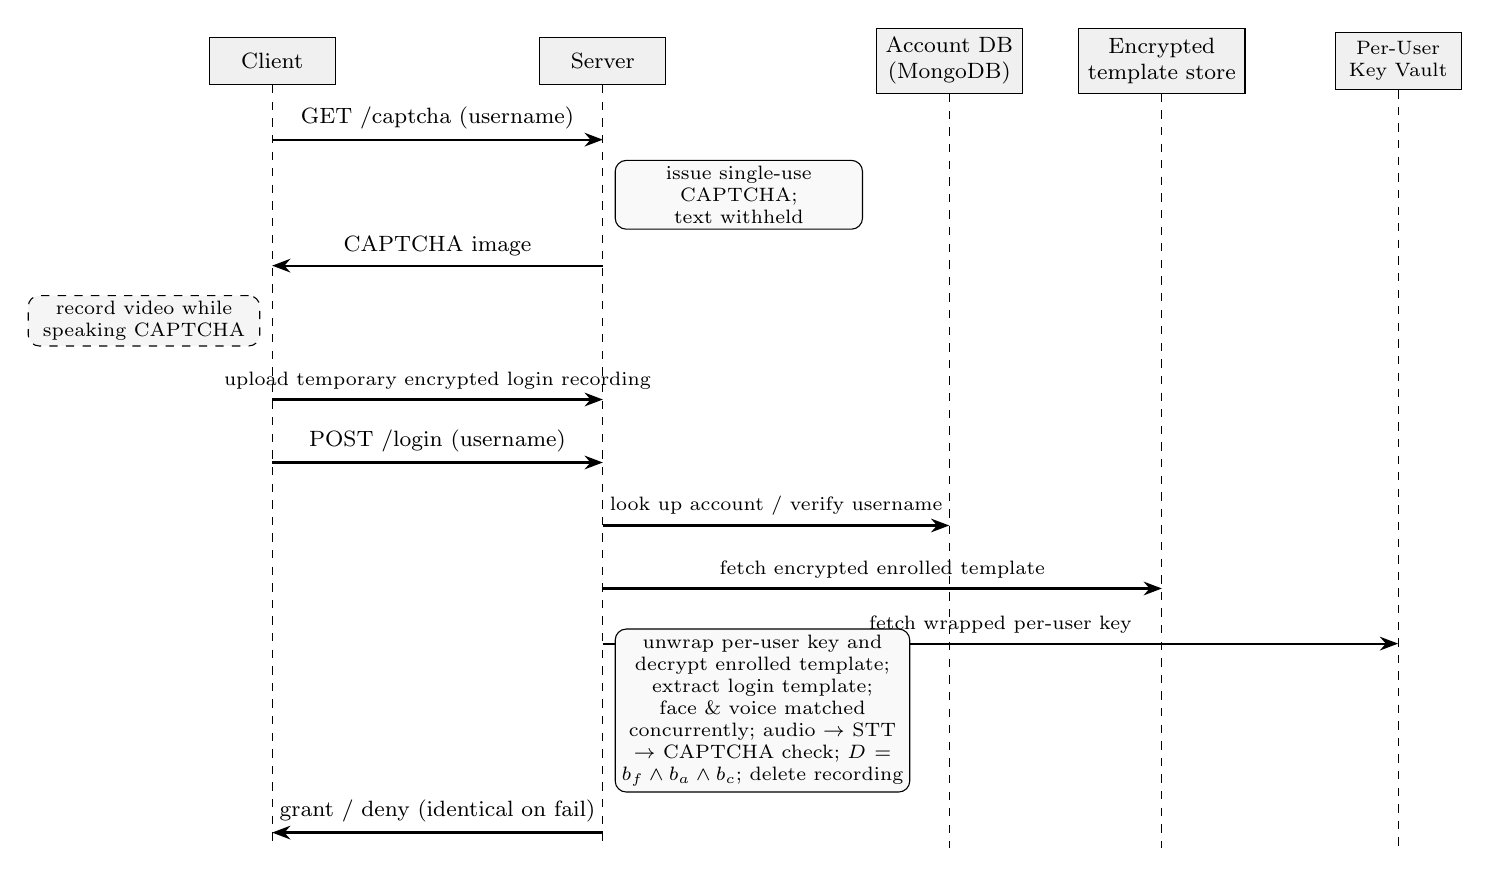
\begin{tikzpicture}[font=\footnotesize, >={Stealth[]},
hdr/.style={draw, fill=gray!12, minimum width=16mm, minimum height=6mm, align=center},
msg/.style={->, thick},
note/.style={draw, fill=gray!5, rounded corners, align=center, inner sep=2pt, font=\scriptsize},
cnote/.style={draw, dashed, fill=gray!8, rounded corners, align=center, inner sep=2pt, font=\scriptsize}]
\node[hdr] (C) at (0,0) {Client};
\node[hdr] (S) at (4.2,0) {Server};
\node[hdr] (M) at (8.6,0) {Account DB\\(MongoDB)};
\node[hdr] (T) at (11.3,0) {Encrypted\\template store};
\node[hdr, font=\scriptsize] (K) at (14.3,0) {Per-User\\Key Vault};
\draw[dashed] (C.south) -- (0,-10.0);
\draw[dashed] (S.south) -- (4.2,-10.0);
\draw[dashed] (M.south) -- (8.6,-10.0);
\draw[dashed] (T.south) -- (11.3,-10.0);
\draw[dashed] (K.south) -- (14.3,-10.0);
\draw[msg] (0,-1) -- node[above]{GET /captcha (username)} (4.2,-1);
\node[note, anchor=west, text width=30mm] at (4.35,-1.7) {issue single-use CAPTCHA; text withheld};
\draw[msg] (4.2,-2.6) -- node[above]{CAPTCHA image} (0,-2.6);
\node[cnote, anchor=east, text width=28mm] at (-0.15,-3.3) {record video while speaking CAPTCHA};
\draw[msg] (0,-4.3) -- node[above, font=\scriptsize]{upload temporary encrypted login recording} (4.2,-4.3);
\draw[msg] (0,-5.1) -- node[above]{POST /login (username)} (4.2,-5.1);
\draw[msg] (4.2,-5.9) -- node[above, font=\scriptsize]{look up account / verify username} (8.6,-5.9);
\draw[msg] (4.2,-6.7) -- node[above, font=\scriptsize]{fetch encrypted enrolled template} (11.3,-6.7);
\draw[msg] (4.2,-7.4) -- node[above, font=\scriptsize]{fetch wrapped per-user key} (14.3,-7.4);
\node[note, anchor=west, text width=36mm] at (4.35,-8.25) {unwrap per-user key and decrypt enrolled template; extract login template; face \& voice matched concurrently; audio $\to$ STT $\to$ CAPTCHA check; $D=b_f\wedge b_a\wedge b_c$; delete recording};
\draw[msg] (4.2,-9.8) -- node[above]{grant / deny (identical on fail)} (0,-9.8);
\end{tikzpicture}
\caption{\textcolor{black}{Login and authentication phase (deployed)}}
\label{fig:5}
\end{figure}

{\color{black}
\begin{algorithm}[H]
\caption{\textcolor{black}{Login and Challenge Issuance}}\label{alg:challenge}
\begin{algorithmic}[1]
\small
\Require identifier $u$
\Ensure a fresh challenge and encrypted login recording

\State Validate identifier $u$; reject if invalid
\State $C \gets$ randomly generate a five-symbol challenge
\State Store $(u,C,\texttt{expiry}=\text{now}+5\text{ min})$
\State Render and send the challenge image to the client
\State User records $V_l$ while speaking $C$
\State Client uploads $V_l$
\State Validate the upload and identifier; reject if invalid
\State Verify that an unexpired challenge exists for $u$; reject otherwise
\State Store $V_l$ in encrypted transient storage
\State Client requests authentication for $u$
\end{algorithmic}
\end{algorithm}
}

\subsection{Authentication Phase}
{\color{black}
\noindent The authentication phase operates on the enrolled biometric template and a newly submitted login recording. Raw enrolment recordings are not retained, while the login recording is stored only temporarily in encrypted form and deleted after the authentication attempt. The three factors are evaluated concurrently as follows.
\begin{enumerate}
\item The submitted identifier is checked against the user accounts.
\item The challenge issued for the identifier is retrieved and consumed, preventing its reuse in a subsequent authentication attempt regardless of the outcome.
\item The enrolled biometric template and encrypted transient login recording are decrypted into a private working directory. Failure to retrieve the user's key, decrypt, or authenticate either protected artefact rejects the attempt.
\item The login recording is processed once to obtain the login representations, consisting of per frame face embeddings and a speaker embedding.
\item The face and voice factors are scored against the enrolled template concurrently using~(\ref{eq:face}) and~(\ref{eq:voice}).
\item Concurrently, the challenge branch extracts the login audio, transcribes it, and evaluates~(\ref{eq:captcha}). This branch operates independently of the biometric matching branch.
\item The three verdicts are combined using the conjunctive rule in~(\ref{eq:fusion}). On success, a signed session token is issued, on authentication failure, the response does not reveal which factor failed.
\item The private working directory and the transient encrypted login recording are removed regardless of the outcome.
\end{enumerate}
}
\begin{table}[!t]
\caption{Challenge, grant, and account lifetimes. The implemented ordering is unenrolled account grace (15 min) $>$ enrollment and re enrollment grant TTL (10 min) $>$ login CAPTCHA TTL (5 min), so cleanup cannot remove an account while its enrollment grant remains valid.}
\label{tab:lifetimes}
\centering
\footnotesize
\renewcommand{\arraystretch}{1.15}
\setlength{\tabcolsep}{4pt}
\begin{tabular}{|p{3.2cm}|p{2.2cm}|p{7.4cm}|}
\hline
\textbf{Artefact} & \textbf{Lifetime} & \textbf{Use and single use constraint} \\ \hline
Login challenge $C$ & 5 min & Single use; consumed on retrieval regardless of outcome \\ \hline
Enrollment grant $E$ & 10 min & Bound to one account with purpose \texttt{enroll}; cannot replace an existing template \\ \hline
Re enrollment grant & 10 min & Bound to one account with purpose \texttt{reenroll}; issued only after successful three factor authentication and may replace only an existing template \\ \hline
Unenrolled account grace & 15 min & Rechecks template presence immediately before cleanup \\ \hline
Session token & Configuration dependent & Lifetime follows the signing environment configuration \\ \hline
\end{tabular}
\end{table}


{\color{black}
\subsection{\textcolor{black}{Threat Model}}\label{sec:threat}
Face and voice are \emph{observable} traits, not secrets: anyone who has met the user, or found them in a public video, holds a sample. No security property below depends on an adversary lacking the victim's face or voice. We define four adversaries and state what each obtains.

\paragraph{A1: holds recordings of the victim.} Archived video and audio of the victim, in any quantity, and the ability to submit arbitrary media to the login endpoint. A1 cannot answer an unpredictable prompt in real time. Both biometric factors \emph{accept}, because the recording genuinely is the victim; the challenge factor rejects, because the archived recording answers a challenge issued in some earlier session while the challenge issued now is fresh and independent of it. Under~(\ref{eq:fusion}) the attempt is denied. This rests on challenge freshness and single use alone --- the system has no liveness or presentation attack detector --- and is measured in Section~\ref{sec:attacks}.

\paragraph{A2: steals the template database.} Read access to every stored template ciphertext and to the account store, but not to the key vault. The templates are AES-256-GCM ciphertexts under per user keys that are not in the stolen material, and each is filed under a keyed pseudonym rather than a username, so the dump does not even reveal whose template is whose. A2 obtains ciphertext. Because keys are per user there is no single key whose compromise unlocks the set, and because the GCM tag authenticates the template, an adversary who can \emph{write} to the store causes a refused login rather than a forged acceptance.

\paragraph{A3: steals the key vault.} Read access to every wrapped per user key and the pseudonymous index, but not to the template store and not to the server side master key. Each row is a wrapped key, useless without the master key and useless anyway without the matching ciphertext held in a different database. Recovering one template requires \emph{both} stores \emph{and} the master key; the deployment refuses to start in production if those secrets are missing, weak, or shared with one another.

\paragraph{A4: controls the network.} Observes and modifies traffic, and may phish, relay, or replay. Transport security is assumed; without it no factor is confidential and this model does not apply. Given it: the challenge text never reaches the client --- only a rendered image does --- so observing a response does not reveal the expected value for a later attempt; the challenge is consumed on retrieval whether or not the attempt succeeds, so a captured upload cannot be resubmitted; and the decision is taken server side, so a modified client cannot assert a verdict.

\paragraph{Why replay fails, quantitatively.} The challenge is five symbols over a ten symbol alphabet, giving $10^{5}=\AttackChallengeSpace$ values, about $16.6$ bits. An archived recording carries a code chosen independently of the one issued now, so it satisfies the challenge factor with probability $10^{-5}$ per attempt. The challenge is \emph{single use}: it is consumed on retrieval regardless of outcome, so each issued challenge admits exactly one guess, and the five minute lifetime bounds how long that guess remains submittable rather than how many guesses are possible. An adversary who requests $n$ fresh challenges and gambles once on each passes the challenge factor with probability $1-(1-10^{-5})^{n}$, about $10^{-3}$ at $n=100$, and must still pass both biometric factors on the same attempt. Raising the entropy is the obvious lever, but the code must be read aloud and transcribed, and Section~\ref{sec:accuracy} shows the challenge factor's false rejections are already the dominant cost to legitimate users.

\paragraph{Template inversion.} What is stored is not a raw face or recording, but neither is it a cancelable template, and we do not claim otherwise. The stored values are deep embeddings, and embeddings of this kind are invertible to a useful degree: reconstruction attacks recover from an embedding alone a face image recognisable to humans and to matchers, and the template protection literature~\cite{rathgeb2023btp,zhao2023deephash} treats an unprotected deep embedding as sensitive data rather than as a one way digest. The protection here is therefore \emph{encryption, not irreversibility}: an adversary holding the plaintext embedding can attempt inversion, and the design's answer is that obtaining the plaintext requires defeating both A2 and A3 together. A true cancelable or deep hashing scheme~\cite{zhao2023deephash} would additionally make a template revocable and unlinkable across deployments; here, unlinkability holds only at the level of \emph{naming}, and revocation means deleting the account and enrolling again.

\paragraph{Out of scope.} A real time relay that presents the live challenge to the victim and returns their response within the validity window defeats the challenge factor by construction, since the response genuinely is fresh and genuinely is the victim; nothing in this design prevents it. A real time responsive deepfake able to generate the victim's face and voice while speaking an unpredictable challenge is likewise out of scope, as are verifier compromise, simultaneous compromise of both stores and the master key, coercion of the enrolled user, and operator abuse. The scheme claims resistance to reuse of previously captured media and states no claim about these.
}

\technicalsubsections
\renewcommand{\algorithmicrequire}{\textbf{Input:}}
\renewcommand{\algorithmicensure}{\textbf{Output:}}

\recentcomparison

\subsection{Account Lifecycle}\label{sec:lifecycle}
The security relevant part of the lifecycle is which operations may create or replace a biometric template, and under what authority. Initial enrollment is authorised by a purpose bound \texttt{enroll} grant and cannot overwrite an existing template; replacement is available only through a \texttt{reenroll} grant, which is issued after the same three factor verification used for login and uses a freshly generated per user key with an atomic ciphertext swap, so a failure before completion leaves the prior enrollment intact. Account deletion erases the record, the encrypted template, the separate vault entry, and any transient recording together. An account that never completed enrollment holds no template and is released automatically after a grace period that deliberately exceeds the enrollment grant lifetime, which in turn exceeds the challenge lifetime (Table~\ref{tab:lifetimes}), so cleanup cannot remove an account while a usable grant for it still exists. Recovery for a user who can no longer authenticate is not exposed as an endpoint at all: an operator verifies identity out of band and deletes the account so the user can enroll again, which makes that administrative procedure --- rather than any cryptographic mechanism --- the recovery trust anchor.

\section{Evaluation and Results}\label{sec:eval}

\subsection{Experimental Setup}
A proof of concept web application was implemented to validate the feasibility of the proposed scheme under real time acquisition. The prototype follows a client--server architecture in which the client performs media acquisition and displays the server issued challenge, while enrolment processing, challenge generation, feature extraction, matching, and decision fusion are performed on the server. Keeping the decision logic server side prevents a modified client from directly bypassing authentication checks.

\subsubsection{Hardware Requirements}\label{sec:hw}
Functional verification was performed on a machine equipped with an Intel Core i5-4210U processor and 8\,GB of RAM. The processing-time measurements reported in Section~\ref{sec:perf} were collected on a separate machine equipped with an Intel Core i9-12900 processor and 62\,GB of RAM. The reported timing results should therefore be interpreted with respect to the second machine.

\subsubsection{Prototype Architecture}
The implementation uses a React single page client, an Express server on Node.js~22, MongoDB for account and storage data, and Python~3.12 for the biometric pipeline. Face inference is performed through ONNX Runtime, while speaker processing uses PyTorch. Production deployments require independent secrets for token signing, biometric storage, and account/PII protection. The server validates these secrets at startup and rejects missing, insecure, or improperly shared production configuration.

{\color{black}

\subsection{\textcolor{black}{Processing and Storage Footprint}}\label{sec:perf}
\subsubsection{Controlled Processing Time}
Controlled per stage processing time was measured over $N=5$ successful genuine authentication runs on the timing machine described in Section~\ref{sec:hw}. Additional live deployment measurements are reported separately in Table~\ref{tab:stages} using the sample counts shown in the table.

\begin{table}[!t]
\caption{\textcolor{black}{Measured per stage processing time (ms). Controlled rows use five successful genuine authentication runs on the i9-12900 timing machine. Live rows use the deployed server benchmark log for four successful logins from the 25 attempts recorded on August 22, 2026; they include ordinary system contention. Both sets show that template extraction dominates and matching contributes comparatively little latency.}}
\label{tab:stages}
\centering
\renewcommand{\arraystretch}{1.27}
\setlength{\tabcolsep}{6pt}
\footnotesize
\begin{tabular}{|>{\raggedright\arraybackslash}p{5.4cm}|c|c|c|c|>{\raggedright\arraybackslash}p{4.3cm}|}
\hline
\rule{0pt}{2.8ex}
\textbf{Stage} &
\textbf{Mean} &
\textbf{Min} &
\textbf{Max} &
\textbf{$N$} &
\textbf{Source} \\
\hline
Login template extraction & 12424 & 11888 & 12779 & 5 & Controlled runs, i9-12900 \\
Face matching             & 98    & 73    & 116   & 5 & Controlled runs \\
Voice matching            & 104   & 83    & 138   & 5 & Controlled runs \\
Audio demultiplexing      & 154   & 146   & 162   & 5 & Controlled runs \\
Speech to text            & 2367  & 2085  & 2666  & 5 & Controlled runs \\
\textbf{Template decryption} & \textbf{9.4} & \textbf{2.6} & \textbf{28.8} & \textbf{4} & \textbf{Live log, successful logins} \\
\textbf{Login template extraction, live} & \textbf{6596} & \textbf{4606} & \textbf{12190} & \textbf{4} & \textbf{Live log, successful logins} \\
\textbf{Face and voice matching, combined, live} & \textbf{150} & \textbf{143} & \textbf{155} & \textbf{4} & \textbf{Live log, successful logins} \\
\textbf{Speech to text, live} & \textbf{2354} & \textbf{1534} & \textbf{3648} & \textbf{4} & \textbf{Live log, successful logins} \\
\textbf{Server side verification, total, live} & \textbf{6746} & \textbf{4757} & \textbf{12339} & \textbf{4} & \textbf{Live log, successful logins} \\
\hline
\end{tabular}
\end{table}

Login template extraction is the dominant processing stage because it loads and executes both the face and speaker model stacks. Model loading contributes substantially to this overhead. By comparison, face and voice matching require only similarity computations between extracted and enrolled representations and introduce comparatively low overhead.

\emph{Storage footprint.} The persistent per user biometric artefact is approximately 147\,KB, while the source recording used for this measurement was 11.18\,MB, an approximately 76 fold difference for that recording. The ratio depends on recording duration, resolution, frame rate, and codec and is therefore reported only as a deployment storage measurement, not as a generic security, accuracy, or comparative advantage. Template storage is $O(1)$ with respect to recording length because the stored representation has fixed dimensions: twelve 512 dimensional face embeddings, one 512 dimensional mean face reference, and one 192 dimensional speaker embedding. The AES 256 GCM envelope adds a fixed 34 byte overhead. Network upload time was not measured and is therefore not reported as an experimental result.

\subsubsection{End-to-End Authentication and Enrollment Timing}
Table~\ref{tab:endtoend} reports user visible registration and authentication timing from the development deployment, separating client pre-upload time from server processing time.

\begin{table}[!t]
\caption{\textcolor{black}{End to end authentication and enrollment time from the deployed development log ($N=25$ attempts). Client pre-upload time includes recording the video and speaking the challenge. For successful login, this user time is approximately 20 seconds of the approximately 27 second total, while mean server processing is 6.76 seconds.}}
\label{tab:endtoend}
\centering
\renewcommand{\arraystretch}{1.18}
\setlength{\tabcolsep}{3.5pt}
\footnotesize
\begin{tabular}{|>{\raggedright\arraybackslash}p{3.6cm}|c|c|c|c|c|c|c|}
\hline
\textbf{Operation} & \textbf{Outcome} & \textbf{$N$} & \textbf{Total mean (s)} & \textbf{Total min (s)} & \textbf{Total max (s)} & \textbf{Client pre-upload mean (s)} & \textbf{Server mean (s)} \\ \hline
Registration, account and enrollment & success & 7 & 11.56 & 7.35 & 14.30 & 1.55 & 10.01 \\ \hline
Login & success & 4 & 26.89 & 14.87 & 42.78 & 20.13 & 6.76 \\ \hline
Login & failure & 13\textsuperscript{*} & 35.08 & 0.02 & 140.08 & 21.13 & 12.95 \\ \hline
\multicolumn{8}{l}{\footnotesize \textsuperscript{*}The log contains 14 failed login records; one has no total because it was rejected before any upload.}
\end{tabular}
\end{table}

These observations complement the controlled per stage measurements by reporting the complete workflow experienced during registration and login.

\subsubsection{Operational Deployment Outcomes}\label{sec:outcomes}
The development deployment recorded 7 successful registrations and 4 successful logins among the 25 logged attempts. The remaining login outcomes comprised 7 \texttt{NO\_ENROLLMENT} records, 6 \texttt{CAPTCHA\_MISMATCH} records, and 1 \texttt{SPEECH\_NOT\_RECOGNIZED} record. These are workflow observations rather than biometric error rates: no logged failure was a biometric mismatch, so no FAR or FRR is inferred from them.

They do, however, locate the system's practical weak point. Of the 11 attempts that reached the challenge branch at all --- the 4 successes plus the 7 challenge failures --- 7, or $63.6\%$, failed there, and \emph{none} failed on face or voice. Under a conjunctive rule every such failure is a denied login for a legitimate user. The third factor, not the biometrics, is what costs this deployment its usability, which is why Section~\ref{sec:accuracy} measures the challenge factor's false rejection rate under controlled conditions rather than leaving it as an incidental log observation.

\subsubsection{Voice Threshold Derivation}
The available diagnostic observations produced a maximum real impostor cosine of 0.256 and a genuine floor of 0.345 after excluding the documented near silent window. The selected voice operating point is $\tau_a=0.30$, as summarized in Table~\ref{tab:voiceevidence}.

\begin{table}[!t]
\caption{Pilot observations from which the voice operating point was originally chosen, reported as threshold provenance. Section~\ref{sec:accuracy} supersedes these with corpus level measurements.}
\label{tab:voiceevidence}
\centering
\renewcommand{\arraystretch}{1.18}
\setlength{\tabcolsep}{6pt}
\footnotesize
\begin{tabular}{|>{\raggedright\arraybackslash}p{6.8cm}|>{\raggedright\arraybackslash}p{4.7cm}|>{\raggedright\arraybackslash}p{4.9cm}|}
\hline
\textbf{Statistic} & \textbf{Value} & \textbf{Basis} \\ \hline
Real cross-speaker impostor cosine, maximum & 0.256 & Pilot diagnostic observations \\ \hline
Genuine same-speaker cosine, floor & 0.345, excluding one near-silent 4 second window & Pilot diagnostic observations \\ \hline
Selected operating point $\tau_a$ & 0.30 & Midpoint of the observed gap \\ \hline
Superseded MFCC statistic, genuine range & 172.8 to 178.8 & Pilot diagnostic observations \\ \hline
Superseded MFCC statistic, impostor range & 153.7 to 193.0; spans the genuine range & Pilot diagnostic observations \\ \hline
\end{tabular}
\end{table}

These pilot observations are what the deployed thresholds were originally chosen from, and they are reported here as provenance only. Section~\ref{sec:accuracy} supersedes them with a corpus level evaluation and revisits both thresholds against it.
}

{\color{black}

\subsection{Recognition Accuracy}\label{sec:accuracy}

\subsubsection{Corpus and pairing protocol.}
Template only storage means the deployment's own enrolment recordings are destroyed after extraction and can never be re-scored, so recognition accuracy is evaluated on an external corpus. We use \EvalCorpusName, a public audio visual dataset whose participants consented to open research release; no new human subject collection was undertaken for this evaluation and no separate ethics approval was therefore required. The corpus contributes \EvalSubjects{} subjects with \EvalSessions{} sessions each. Because the deployed speaker model is itself trained on a public speaker corpus, the evaluation corpus is chosen to be disjoint from that training data; a corpus overlapping it would score the model on material it has already seen, and the harness records and reports the overlap verdict for whatever corpus is used.

Pairs are formed exactly as the deployed matchers would score them. A \emph{genuine} pair compares two \emph{different sessions of the same subject}; a recording is never compared with itself, since a self comparison scores $1.0$ and would deflate the false rejection rate. An \emph{impostor} pair compares recordings of different subjects. This yields \EvalGenuinePairs{} genuine and \EvalImpostorPairs{} impostor pairs. For a threshold $\tau$, $\mathrm{FAR}(\tau)=P(s\geq\tau\mid\text{impostor})$ and $\mathrm{FRR}(\tau)=P(s<\tau\mid\text{genuine})$, and the Equal Error Rate is the common error value at the threshold where the two are equal.

\subsubsection{Face, voice, and the fused decision.}
Table~\ref{tab:accuracy} reports EER, AUC, the threshold at the EER, and FAR and FRR at the deployed operating points, for each factor and for the conjunctive decision. Figure~\ref{fig:roc} gives the ROC and DET curves and Figure~\ref{fig:scoredist} the genuine and impostor score distributions, with both the deployed and the EER threshold marked.

\begin{table}[!t]
\caption{Recognition accuracy on \EvalCorpusName. Genuine pairs are formed only between different sessions of the same subject; impostor pairs between different subjects. The challenge factor is not a biometric trial and has no impostor pair structure, so only its false rejection rate is defined.}
\label{tab:accuracy}
\centering
\renewcommand{\arraystretch}{1.18}
\setlength{\tabcolsep}{4pt}
\footnotesize
\begin{tabular}{lrrrrrrr}
\toprule
\textbf{Modality} & \textbf{Gen.} & \textbf{Imp.} & \textbf{EER (\%)} & \textbf{AUC} & \textbf{FAR (\%)} & \textbf{FRR (\%)} & \textbf{$\tau$ at EER} \\
\midrule
\EvalAccuracyRows
\bottomrule
\end{tabular}
\end{table}

% The figures are produced by the evaluation harness alongside results.tex. The
% \IfFileExists guards keep the document compiling before a corpus run, rather
% than failing on a missing graphic.
\begin{figure}[!t]
\centering
\IfFileExists{fig_roc.png}{\includegraphics[width=0.48\textwidth]{fig_roc.png}}{\fbox{\parbox{0.45\textwidth}{\centering\vspace{2em}\textit{fig\_roc.png: produced by the evaluation harness}\vspace{2em}}}}
\hfill
\IfFileExists{fig_det.png}{\includegraphics[width=0.48\textwidth]{fig_det.png}}{\fbox{\parbox{0.45\textwidth}{\centering\vspace{2em}\textit{fig\_det.png: produced by the evaluation harness}\vspace{2em}}}}
\caption{ROC (left) and DET (right) curves for the face and speaker factors on \EvalCorpusName.}
\label{fig:roc}
\end{figure}

\begin{figure}[!t]
\centering
\IfFileExists{fig_score_dist.png}{\includegraphics[width=0.95\textwidth]{fig_score_dist.png}}{\fbox{\parbox{0.9\textwidth}{\centering\vspace{2em}\textit{fig\_score\_dist.png: produced by the evaluation harness}\vspace{2em}}}}
\caption{Genuine and impostor cosine similarity distributions for the face (left) and speaker (right) factors. The dashed line marks the deployed threshold and the dash-dotted line the threshold at the EER; the distance between them is the operating margin discussed in the text.}
\label{fig:scoredist}
\end{figure}

\subsubsection{Re-justifying the thresholds.}
The deployed operating points were inherited ($\tau_f=0.35$) and chosen from a handful of pilot observations ($\tau_a=0.30$), before any corpus level measurement existed. The corpus places the face EER at $\tau=\EvalFaceEERTau$ and the voice EER at $\tau=\EvalVoiceEERTau$. Where a deployed threshold sits away from its modality's EER threshold, that is a deliberate asymmetry rather than an oversight: this is an \emph{authentication} system under a conjunctive rule, in which a false acceptance admits an impostor while a false rejection merely asks the user to try again, so operating on the strict side of the EER is the correct trade. What the EER threshold provides is the reference point that makes the size of that asymmetry visible and arguable, which the pilot observations could not.

\subsubsection{The challenge factor's own error rate.}
The third factor is the one that most often rejects a legitimate user, and it is not captured by any biometric pair. We measure it separately over \EvalChallengeTrials{} controlled trials in which the speaker reads a known code correctly, so that \emph{every} rejection is by construction a false rejection. The measured challenge false rejection rate is \EvalChallengeFRR\%, decomposed into transcriptions that returned the wrong string and transcriptions that returned nothing at all. This is consistent with the deployment log of Section~\ref{sec:outcomes}, where the challenge branch accounted for every observed login failure that reached it.

\subsubsection{Does AND fusion behave independently?}
Equations~(\ref{eq:farsys}) and~(\ref{eq:frrsys}) predict the fused error only if the factors fail independently. Table~\ref{tab:independence} compares the prediction with the measured fused error.

\begin{table}[!t]
\caption{Measured conjunctive fusion against the independence approximation of~(\ref{eq:farsys}) and~(\ref{eq:frrsys}). A measured value above the prediction indicates positively correlated failures.}
\label{tab:independence}
\centering
\renewcommand{\arraystretch}{1.18}
\footnotesize
\begin{tabular}{lrrr}
\toprule
& \textbf{Predicted (\%)} & \textbf{Measured (\%)} & \textbf{Difference (\%)} \\
\midrule
\EvalIndependenceRows
\bottomrule
\end{tabular}
\end{table}

The comparison is informative in either direction. All three factors are derived from a single recording, so a capture that is dark, short, or noisy can degrade more than one of them at once; where the measured false rejection exceeds the prediction, that common cause is visible, and the independence form should be read as a design heuristic rather than as a model of this system's error behaviour.

\subsubsection{Cross-device behaviour.}
The capture client records the negotiated width, height, frame rate and platform for every attempt, so genuine pairs can be split by whether the two sessions came from the same device class. Table~\ref{tab:crossdevice} reports the split. Where the corpus provides only one device condition, the split is not reported rather than being approximated: a single device corpus cannot support a cross device claim, and the harness refuses to emit one.

\begin{table}[!t]
\caption{Genuine score behaviour within and across device classes, at the deployed thresholds. Impostor pairs are pooled, since two different people do not match regardless of what recorded them.}
\label{tab:crossdevice}
\centering
\renewcommand{\arraystretch}{1.18}
\footnotesize
\begin{tabular}{lrrrr}
\toprule
& \multicolumn{2}{c}{\textbf{Within device}} & \multicolumn{2}{c}{\textbf{Across devices}} \\
\cmidrule(lr){2-3}\cmidrule(lr){4-5}
\textbf{Modality} & \textbf{Genuine mean} & \textbf{FRR (\%)} & \textbf{Genuine mean} & \textbf{FRR (\%)} \\
\midrule
\EvalCrossDeviceRows
\bottomrule
\end{tabular}
\end{table}

\subsection{Attack Evaluation}\label{sec:attacks}
Each attack is mounted against the deployed pipeline: the same template extractor, the same two matchers at the same thresholds, the same transcription and normalisation, and the conjunctive rule of~(\ref{eq:fusion}). Attack media is synthesised from a consented corpus of \AttackSubjects{} subjects recorded reading known five symbol codes, which is necessary because the challenge factor cannot be scored against a recording whose spoken content is unknown. Every run includes a control: a genuine attempt by the victim against the challenge their own recording speaks. The control must be accepted, since a harness that rejects everything would report zero attack success whether or not it worked, and no attack figures are reported from a run whose control failed.

Table~\ref{tab:attacks} reports each attack four ways. The three per factor rates say whether the face, speaker, and challenge factors individually accepted the attack medium; the system rate is the fraction of attempts actually granted access.

\begin{table}[!t]
\caption{Attack success rates against the deployed decision rule. Per factor rates report whether each factor individually accepted the attack medium; the system rate is the fraction granted access under the conjunctive rule.}
\label{tab:attacks}
\centering
\renewcommand{\arraystretch}{1.18}
\setlength{\tabcolsep}{5pt}
\footnotesize
\begin{tabular}{lrrrrr}
\toprule
\textbf{Attack} & \textbf{$n$} & \textbf{Face ASR (\%)} & \textbf{Voice ASR (\%)} & \textbf{Chall.\ ASR (\%)} & \textbf{System ASR (\%)} \\
\midrule
\AttackRows
\bottomrule
\end{tabular}
\end{table}

Table~\ref{tab:attackdefence} maps each attack in the threat model of
Section~\ref{sec:threat} onto the adversary that mounts it, the mechanism that is
supposed to stop it, and what was actually observed. Rows without a measured rate
are design properties rather than trials: a stolen ciphertext either is or is not
decryptable, and there is nothing to sample.

\begin{table}[!t]
\caption{Attack, responsible adversary, defending mechanism, and outcome. Measured rates are system-level attack success rates from Table~\ref{tab:attacks}; \emph{design} rows follow from the construction and are argued rather than sampled. The genuine control was accepted (\AttackControlValid), without which the measured zeros below would be uninformative.}
\label{tab:attackdefence}
\centering
\renewcommand{\arraystretch}{1.15}
\setlength{\tabcolsep}{4pt}
\scriptsize
\begin{tabular}{@{}p{4.1cm}cp{3.6cm}p{3.5cm}@{}}
\toprule
\textbf{Attack} & \textbf{Adv.} & \textbf{Defence mechanism} & \textbf{Result} \\
\midrule
Replay an archived login recording & A1 & Fresh, single-use challenge & \AttackReplayASR\% of \AttackReplayN; bound $1/\AttackChallengeSpace$ per attempt \\
Photograph or screen, attacker speaks the challenge & A1 & Speaker factor \emph{only} (no PAD) & \AttackPhotoLiveVoiceASR\% of \AttackPhotoLiveVoiceN; face factor alone accepts \AttackPhotoLiveVoiceFaceASR\% \\
Photograph plus the victim's archived audio & A1 & Fresh challenge & \AttackPhotoArchivedAudioASR\% of \AttackPhotoArchivedAudioN \\
Victim's face spliced with the attacker's live voice & A1 & Speaker factor & \AttackSpliceVictimFaceASR\% of \AttackSpliceVictimFaceN \\
Attacker's face with the victim's archived voice & A1 & Face factor & \AttackSpliceVictimVoiceASR\% of \AttackSpliceVictimVoiceN \\
Cloned voice answering the live challenge & A1 & Speaker factor \emph{only} & \AttackVoiceCloneASR\% of \AttackVoiceCloneN \\
Face-swapped video with a live spoken answer & A1 & Face factor \emph{only} & \AttackFaceSwapASR\% of \AttackFaceSwapN \\
\midrule
Steal the template store & A2 & Per-user AES-256-GCM; keys held in a separate vault & Ciphertext only \emph{(design)} \\
Steal the key vault & A3 & Master-key wrapping; no ciphertext co-located & Wrapped keys only \emph{(design)} \\
Steal both stores and the master key & A2+A3 & --- & Templates recovered; inversion then plausible \emph{(design)} \\
Tamper with a stored template & A2 & GCM authentication tag & Login refused, not evaluated \emph{(design)} \\
Overwrite an enrolled template via registration & A1 & Purpose-bound \texttt{enroll} grant & Rejected \emph{(design)} \\
Replace a template without authenticating & A1 & \texttt{reenroll} grant, issued only after three-factor success & Rejected \emph{(design)} \\
\midrule
Real-time relay of the live challenge & A1, A4 & --- & \textbf{Out of scope; succeeds} \\
Real-time responsive deepfake & A1 & --- & \textbf{Out of scope; not evaluated} \\
\bottomrule
\end{tabular}
\end{table}

Reporting per factor rates is deliberate, because the system rate alone conceals the mechanism. A photograph held to the camera is accepted by the face factor --- the system has no presentation attack detection, and we do not claim any --- and is denied only because the attacker cannot simultaneously satisfy the speaker factor. Splicing the victim's face onto an attacker's live spoken answer likewise defeats two factors and is stopped by the third. These are the cases in which conjunctive fusion is doing visible work, and they argue for the design more convincingly than an undifferentiated report that no attack succeeded.

Two results deserve to be read without softening. First, the face factor is defeated by trivially available media, so the security of this system rests on the speaker factor and the challenge, not on face verification. Second, synthetic speech attacks the one factor that stops the strongest attacks; whatever success rate the cloning row reports is the most important number in the table, and it is reported as measured. Where an attack succeeds, that is evidence for the anti spoofing work identified in Section~\ref{sec:future}, not a result to be qualified away.

Replay is the one row where the residual risk is argued rather than sampled. A replayed recording satisfies the challenge only if its archived code coincides with the freshly issued one, with probability $1/\AttackChallengeSpace$ per attempt; observing that empirically would require on the order of $10^{5}$ trials to see a single event, so it is derived from the challenge space in Section~\ref{sec:threat} and reported as an analytic bound.

\subsection{\textcolor{black}{Evaluation Scope and Limitations}}\label{sec:limits}
The recognition accuracy evaluation is performed on a public corpus rather than on recordings from the deployment itself, because template only storage destroys enrolment recordings by design. That corpus was captured under its own conditions, which are not those of the deployed capture client, so the reported error rates characterise the deployed \emph{matchers} on a controlled corpus rather than the end to end system under field conditions. Where the corpus offers a single device class, the cross device split in Table~\ref{tab:crossdevice} is withheld rather than estimated.

The attack evaluation covers archived media, splicing, photograph and screen replay, synthetic speech, and face swapping. It does not cover a real time relay or a real time responsive deepfake, both of which are outside the threat model of Section~\ref{sec:threat} and neither of which this design claims to resist. The cloning and face swap rows characterise one off the shelf tool each and should not be read as a bound over all such tools.

Key rotation is not automated and remains an operational limitation. The system separates signing, biometric storage, and account data protection keys, but replacing a storage key currently requires a controlled migration of the protected data; automated key versioning and online re-encryption remain future work.

}
\section{Future Work}\label{sec:future}
A primary direction for future work is to strengthen the proposed authentication system against deepfake and advanced presentation attacks. Although the dynamic CAPTCHA provides challenge response based protection against simple replay attacks, an attacker may potentially use AI generated or manipulated facial and voice content to imitate an enrolled user. Therefore, future work will investigate the integration of dedicated deepfake and presentation attack detection mechanisms for both facial and voice modalities.

For the facial modality, future work can incorporate face anti spoofing and deepfake detection techniques to distinguish genuine live facial input from replayed, manipulated, or synthetically generated video. Similarly, for the voice modality, synthetic speech and voice cloning detection can be integrated to identify AI generated or converted speech. These additional checks can operate alongside the existing face verification, speaker verification, and challenge response mechanisms, providing an additional layer of protection rather than replacing the current authentication factors.

Future work will also focus on evaluating the complete system against a broader range of attack scenarios involving manipulated video, cloned speech, and multimodal deepfakes. The goal will be to determine whether face, voice, and liveness related evidence can be jointly analysed to improve resistance against attacks in which multiple biometric modalities are synthetically generated or manipulated simultaneously.

Two limitations identified by the measurements point to concrete engineering work. Template extraction dominates authentication latency (Table~\ref{tab:stages}) largely because each attempt loads both model stacks from cold; holding the face and speaker models resident in a persistent extraction service removes that load cost from the critical path, and is the single largest available latency reduction. Separately, the challenge factor's false rejections dominate the failures legitimate users actually experience (Sections~\ref{sec:outcomes} and~\ref{sec:accuracy}), which makes the accuracy of the transcription stage --- not the biometrics --- the most valuable usability target, and which also bounds how far the challenge entropy can be raised without making the system harder to use.

A cross device protocol recording each consenting subject in multiple sessions on at least two devices would extend Table~\ref{tab:crossdevice} beyond the device conditions a public corpus happens to provide. Automated key rotation and online re encryption remain operational work. No dedicated facial or voice deepfake detector, and no Presentation Attack Detection model, is claimed as part of the current implementation.

\section{Conclusion}\label{sec:conclusion}
This paper presents a single sensor multimodal biometric authentication system that combines face verification, speaker verification, and a dynamic challenge response mechanism using a single real time video recording. Facial and voice information are acquired simultaneously, while the user responds to a server generated CAPTCHA. Authentication is granted only when all three factors are successfully verified through a conjunctive decision rule.

The implemented system uses deep face embeddings and cosine similarity for face verification, ECAPA-TDNN speaker embeddings and cosine similarity for speaker verification, and speech to text based challenge validation. Raw enrollment recordings are deleted after template extraction, while encrypted login recordings are retained only transiently and deleted when the authentication attempt resolves. The resulting biometric templates are protected and stored separately from account information, supporting a privacy conscious authentication workflow.

\ifresultsready
On \EvalCorpusName, over \EvalGenuinePairs{} genuine pairs formed across different sessions of the same subject and \EvalImpostorPairs{} impostor pairs across different subjects, the face factor attains an EER of \EvalFaceEER\% (AUC \EvalFaceAUC) and the speaker factor \EvalVoiceEER\% (AUC \EvalVoiceAUC); at the deployed thresholds the conjunctive decision gives a FAR of \EvalFusedFAR\% and an FRR of \EvalFusedFRR\%. The challenge factor rejects \EvalChallengeFRR\% of correctly spoken responses, and is the dominant source of failure for legitimate users --- the cost conjunctive fusion imposes in exchange for the false acceptance rate it buys.
\else
Recognition accuracy is measured by an automated harness over genuine pairs formed across different sessions of the same subject and impostor pairs across different subjects, reporting FAR, FRR, EER, AUC, ROC and DET for each factor and for the conjunctive decision, together with the challenge factor's own false rejection rate; the corpus run is outstanding at the time of writing.
\fi
\ifattacksready
Against presentation attacks, replay of archived recordings, face--voice splicing in both directions, photograph and screen replay, synthetic speech and face swapping were mounted against the deployed decision rule and reported per factor as well as for the system. The per factor view is the informative one: the face factor is accepted by media an adversary can obtain trivially, and the system holds because the speaker factor and the fresh challenge cannot be satisfied at the same time from archived material.
\else
A presentation attack harness mounts replay, splicing, photograph and screen replay, synthetic speech and face swapping against the deployed decision rule, reporting per factor and system attack success rates; those runs are outstanding at the time of writing.
\fi
Template extraction remained the dominant processing stage, while face and voice matching introduced comparatively low overhead.

The result is a deployable multimodal authenticator built from commodity camera and microphone hardware, whose security rests on stated and measured properties rather than on assumed ones: a fresh single use challenge worth $1/\AttackChallengeSpace$ per attempt against archived media, conjunctive fusion whose contribution is visible in the per factor attack rates, and encrypted per user templates held separately from their keys. Its limits are equally explicit --- no presentation attack detection, templates that are encrypted rather than cancelable, and no defence against an adversary able to answer the challenge in real time.

\iffalse
```latex
{\color{black}
\begin{algorithm}[!tbp]
\caption{\textcolor{black}{User Registration / Enrolment}}
\label{alg:register}
\begin{algorithmic}[1]
\small
\Require identifier $u$; email $m$; optional avatar; registration recording $V_r$
\Ensure encrypted biometric template or rejection

\State \textbf{Account creation:}
\State validate $u$ and $m$; reject if invalid
\State $\texttt{idx}\gets\mathcal{H}_{k_{\mathrm{pii}}}(\texttt{email-index:}\mathcal{N}_e(m))$
\State $a_u\gets\mathrm{Find}(u)$; $a_m\gets\mathrm{Find}(\texttt{idx})$
\State \textbf{if} $a_u$ or $a_m$ contains an enrolled template \textbf{then reject}
\State delete any existing template-less $a_u,a_m$; create account $(u,\texttt{idx},m,\text{avatar})$
\State $E\gets\mathrm{Sign}_{k_{\mathrm{sig}}}(\{\texttt{username}=u,\texttt{purpose}=\mathrm{enroll}\},\texttt{ttl}=10\text{ min})$
\State \Return $E$

\State \textbf{Biometric enrolment:}
\State client uploads $V_r$ with enrollment token $E$
\State verify $E$; reject if missing, invalid, expired, or malformed
\State $u'\gets$ username claim of $E$
\State $a\gets\mathrm{Find}(u')$
\State \textbf{if} $a$ does not exist, filename is invalid, or $a$ already has a template \textbf{then reject}
\State $T_r\gets\textsc{ExtractTemplate}(V_r)$
\If{$T_r=\textbf{failure}$}
    \State delete temporary data and roll back the template-less account
    \State \Return rejection
\EndIf
\State $C\gets\mathrm{Enc}^{\mathrm{AES\text{-}256\text{-}GCM}}_{k_{\mathrm{bio}}}(T_r)$
\State $\texttt{id}_T\gets\mathcal{H}_{k_{\mathrm{bio}}}(\texttt{template-name:}u')$
\State store $C$ as encrypted template $\texttt{id}_T.\mathrm{tmpl.enc}$
\State delete $V_r,T_r$ and all temporary plaintext data
\State \Return success
\end{algorithmic}
\end{algorithm}






\begin{algorithm}[!tbp]
\caption{\textcolor{black}{Login and Challenge Issuance}}
\label{alg:challenge}
\begin{algorithmic}[1]
\small
\Require identifier $u$
\Ensure server-side challenge $C$ and encrypted transient login recording $V_l$

\State validate $u$; reject if invalid
\State $C\gets$ five random digits from $\{0,\ldots,9\}$
\State store $(u,C,\texttt{expiry}=\mathrm{now}+5\text{ min})$ server-side
\State render $C$ as an SVG and transmit only the SVG to the client
\State client records login video $V_l$ while speaking $C$
\State client uploads $V_l$ with filename $u'\texttt{\_l.mp4}$
\State validate filename; reject if invalid
\State $u'\gets$ identifier extracted from the validated filename
\State \textbf{if} no unexpired challenge exists for $u'$ \textbf{then reject}
\State $C_l\gets\mathrm{Enc}^{\mathrm{AES\text{-}256\text{-}GCM}}_{k_{\mathrm{bio}}}(V_l)$
\State store $C_l$ as a transient encrypted login recording
\State \Return authentication request
\end{algorithmic}
\end{algorithm}





}
\fi
\bibliographystyle{splncs04}
\bibliography{refs}
\end{document}
